\documentclass[10pt]{beamer}
\usetheme{Madrid}
\usecolortheme{default}
\setbeamertemplate{navigation symbols}{}

% Packages
\usepackage[utf8]{inputenc}
\usepackage{graphicx}
\usepackage{amsmath}
\usepackage{amsfonts}
\usepackage{amssymb}
\usepackage{xcolor}
\usepackage{tikz}
\usepackage{pgfplots}
\pgfplotsset{compat=1.18}
\usetikzlibrary{arrows,shapes,positioning}

% Title page information
\title[Robot Localization with ROS]{\texorpdfstring{Robot Localization with ROS: \\Final Presentation (Steps 1–3)}{Robot Localization with ROS: Final Presentation (Steps 1–3)}}
\subtitle{Mini-Project 1 Final Report}
\author{Nicholas Birch de la Calle (IST1116701) \\
Antonio Maria Trigueiros de Arag\~{a}o Moura Coutinho (IST196837) \\
Gabriel Badan (IST1116537) \\
Jana\'{\i}na da Silva Pacheco (IST1117233)}
\institute{Instituto Superior Técnico}
\date{September 24, 2025}

% Title graphic (IST/Técnico logo) — tries common filenames and sibling folders; skips if not found
\IfFileExists{Tecnico Lisbon Logo.jpg}{\titlegraphic{
\includegraphics[height=1.6cm]{Tecnico Lisbon Logo.jpg}}}{%%
\IfFileExists{Tecnico Lisbon Logo.png}{\titlegraphic{
\includegraphics[height=1.6cm]{Tecnico Lisbon Logo.png}}}{%%
\IfFileExists{tecnico.jpg}{\titlegraphic{\includegraphics[height=1.6cm]{tecnico.jpg}}}{%%
\IfFileExists{logo.jpg}{\titlegraphic{\includegraphics[height=1.6cm]{logo.jpg}}}{%%
\IfFileExists{../presentation 1/Tecnico Lisbon Logo.jpg}{\titlegraphic{
\includegraphics[height=1.6cm]{../presentation 1/Tecnico Lisbon Logo.jpg}}}{%%
\IfFileExists{../presentation 1/tecnico.jpg}{\titlegraphic{\includegraphics[height=1.6cm]{../presentation 1/tecnico.jpg}}}{}}}}}}

\begin{document}

% Title slide
\begin{frame}
\titlepage
\end{frame}

% Outline
\begin{frame}{Outline}
\tableofcontents
\end{frame}

% Team & scope
\section{Team \& Scope}

\begin{frame}{Scope for This Week}
\begin{itemize}
    \item \textbf{Step 1 :} Compared \texttt{odom} and \texttt{filtered odometry} against mocap ground truth and evaluated the error
    \item \textbf{Step 2 :} Built a map from the real robot; created a playback \texttt{.bag}
    \item \textbf{Step 3 :} Navigation with Monte Carlo Localization
\end{itemize}
\end{frame}

% Step 1: GT comparison
\section{Step 1: Ground Truth Comparison}

\begin{frame}{Our Method: EKF Sensor Fusion}
\begin{itemize}
    \item We used \textbf{Extended Kalman Filter (EKF)} to combine:
    \begin{itemize}
        \item Wheel odometry (where the robot thinks it is)
        \item IMU data (robot's rotation and acceleration)
        \item Ground truth at 1Hz (like GPS corrections)
    \end{itemize}
    \item Compared 3 trajectories: Raw sensors vs EKF vs True path
    \item Measured errors in real-time (around \textbf{110mm average})
\end{itemize}

\vspace{3mm}
\begin{block}{Real-World Application}
This simulates indoor robots using periodic position updates from WiFi/beacon systems
\end{block}
\end{frame}

\begin{frame}{What We Achieved}
\begin{columns}
\begin{column}{0.6\textwidth}
\begin{itemize}
    \item \textbf{Three trajectories} visualized in real-time:
    \begin{itemize}
        \item Blue: Raw wheel sensors
        \item Red: EKF filtered (our system)
        \item Green: True robot position
    \end{itemize}
    \item \textbf{Error measurement:} ~110mm average
    \item EKF successfully fuses all sensor data
\end{itemize}
\end{column}
\begin{column}{0.38\textwidth}
\centering
\IfFileExists{grouns_truuth_patgh.png}{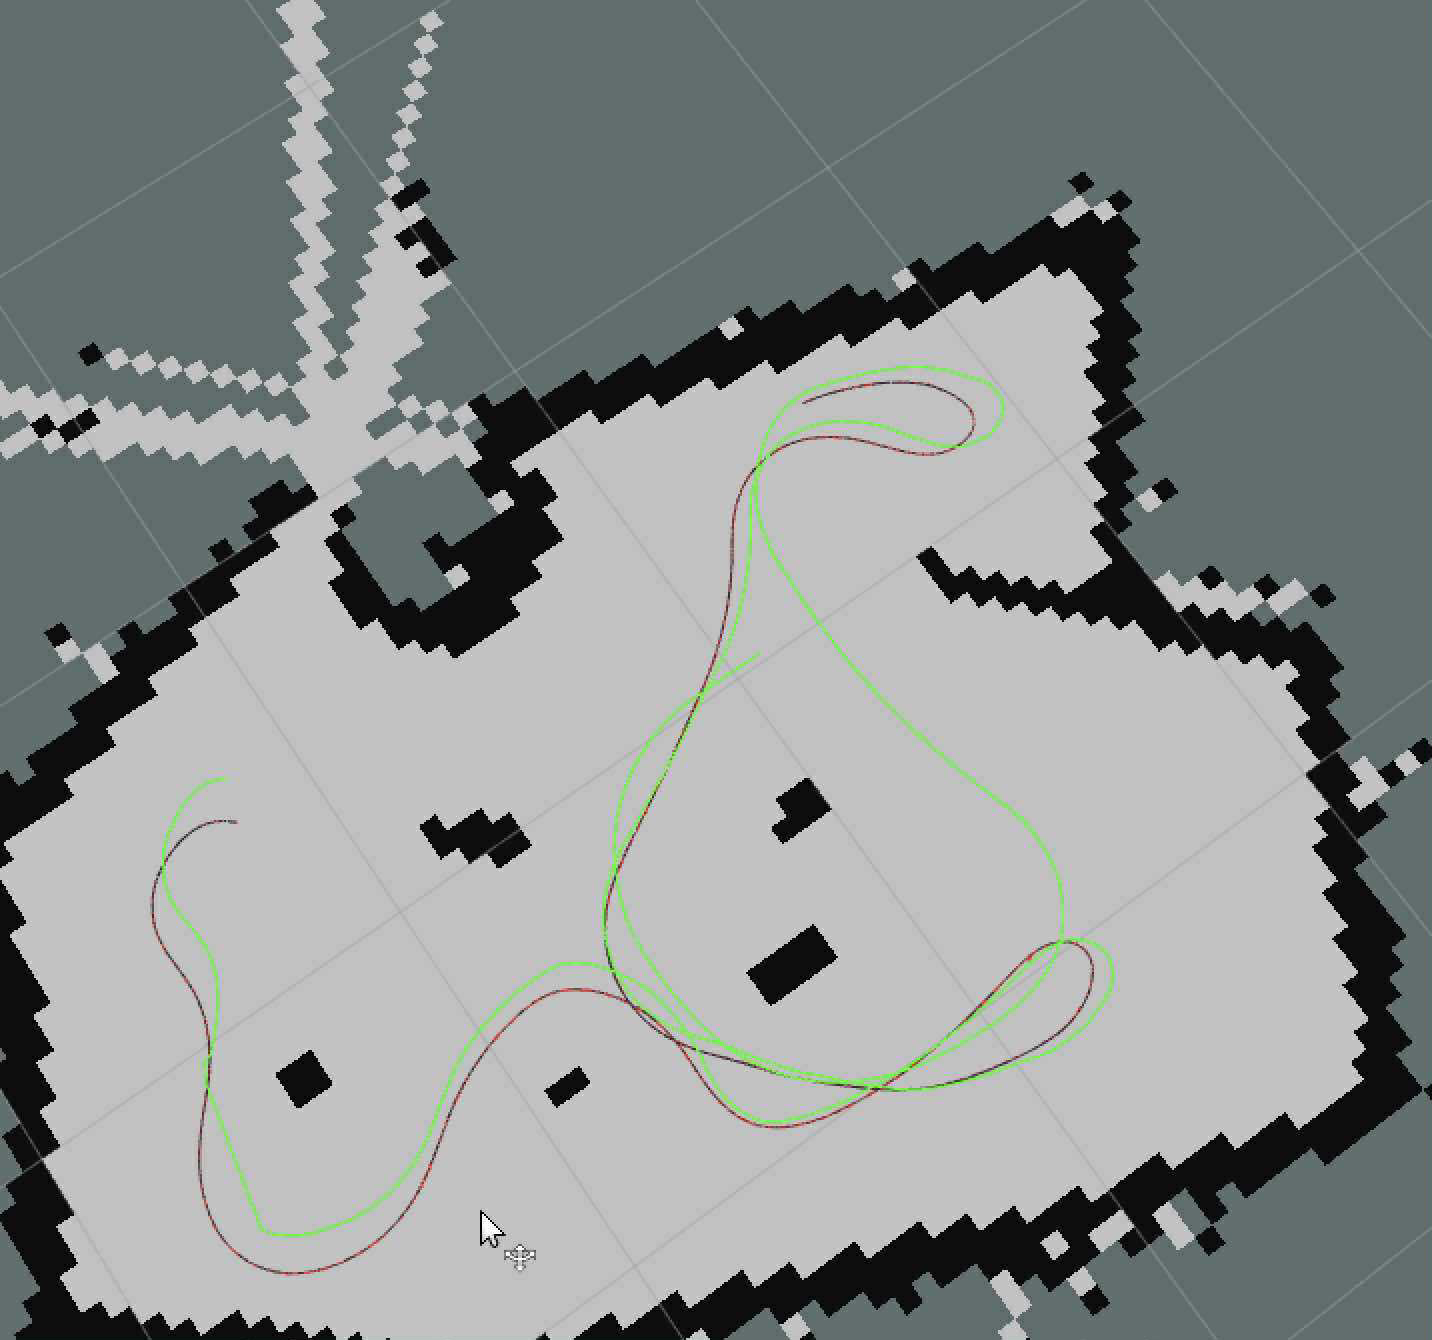
\includegraphics[width=\textwidth]{grouns_truuth_patgh.png}}{\textit{[Ground truth comparison]}}

\vspace{1mm}
{\tiny Three-way comparison showing our EKF system performance}
\end{column}
\end{columns}
\end{frame}

% Step 2: Using the Map
\section{Step 2: Building the Map with gmapping}

\begin{frame}{How gmapping Works}
\begin{itemize}
    \item \textbf{gmapping = SLAM algorithm} (Simultaneous Localization and Mapping)
    \item Uses \textbf{particle filter} where each particle represents a possible robot path
    \item Each particle builds its own version of the map as it moves
    \item \textbf{Laser scans} detect walls and obstacles
    \item \textbf{Wheel odometry} estimates robot movement between scans
\end{itemize}

\vspace{3mm}
\begin{block}{The Process}
\begin{enumerate}
    \item Robot drives around unknown environment
    \item Laser continuously scans surroundings (360°)
    \item Algorithm builds map while tracking robot position
    \item Final result: Complete occupancy grid map
\end{enumerate}
\end{block}
\end{frame}

\begin{frame}{Building the Map}
\begin{itemize}
    \item Built the map using \textbf{live data collection} with the TurtleBot3 robot
    \item Used gmapping SLAM to create occupancy grid from laser scans
    \item Robot navigated the lab environment while simultaneously mapping
    \item Generated map saved for subsequent localization experiments
\end{itemize}

\begin{center}
\IfFileExists{Chat with Nicholas.png}{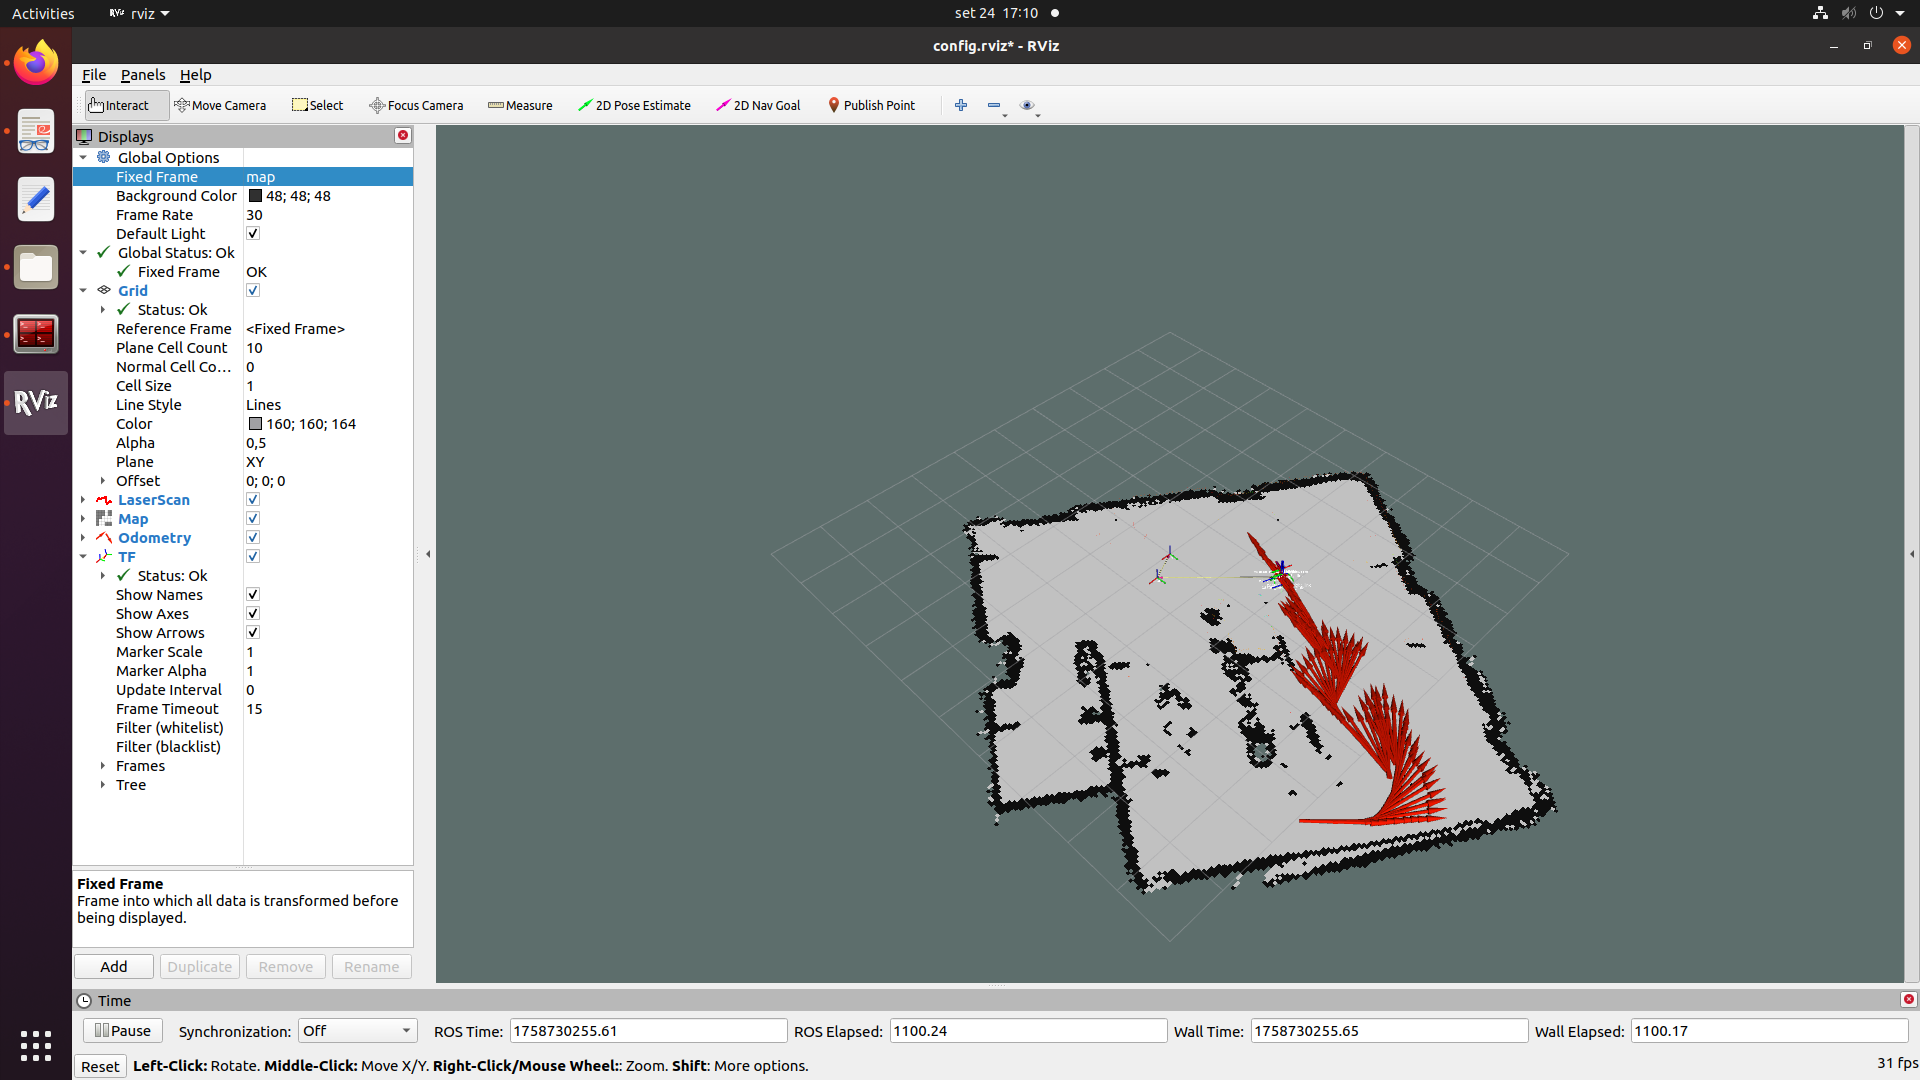
\includegraphics[width=0.7\textwidth]{Chat with Nicholas.png}}{\IfFileExists{map.png}{\includegraphics[width=0.7\textwidth]{map.png}}{\textit{[Lab environment map]}}}
\end{center}
\end{frame}

% Step 3: AMCL Localization
\section{Step 3: AMCL Localization}

\begin{frame}{What is AMCL?}
\begin{itemize}
    \item \textbf{AMCL = Adaptive Monte Carlo Localization}
    \item Uses \textbf{particle filter} to find robot position on the map
    \item Combines laser scans + odometry + map to localize
    \item Each particle represents a possible robot position
\end{itemize}

\vspace{5mm}
\begin{block}{How it Works}
\begin{enumerate}
    \item Scatter particles across the map (possible positions)
    \item Compare laser scans with map at each particle location  
    \item Keep particles that match well, remove bad ones
    \item Converge to the most likely robot position
\end{enumerate}
\end{block}
\end{frame}

\begin{frame}{AMCL Implementation Results}
\begin{columns}
\begin{column}{0.5\textwidth}
\begin{itemize}
    \item Successfully implemented AMCL localization
    \item Particle filter \textbf{converges} to correct position
    \item Robot accurately tracked on the map
    \item System ready for navigation tasks
\end{itemize}

\vspace{3mm}
\textbf{Next Step:} Autonomous navigation with waypoint following (future work)
\end{column}
\begin{column}{0.48\textwidth}
\centering
\IfFileExists{image.jpg}{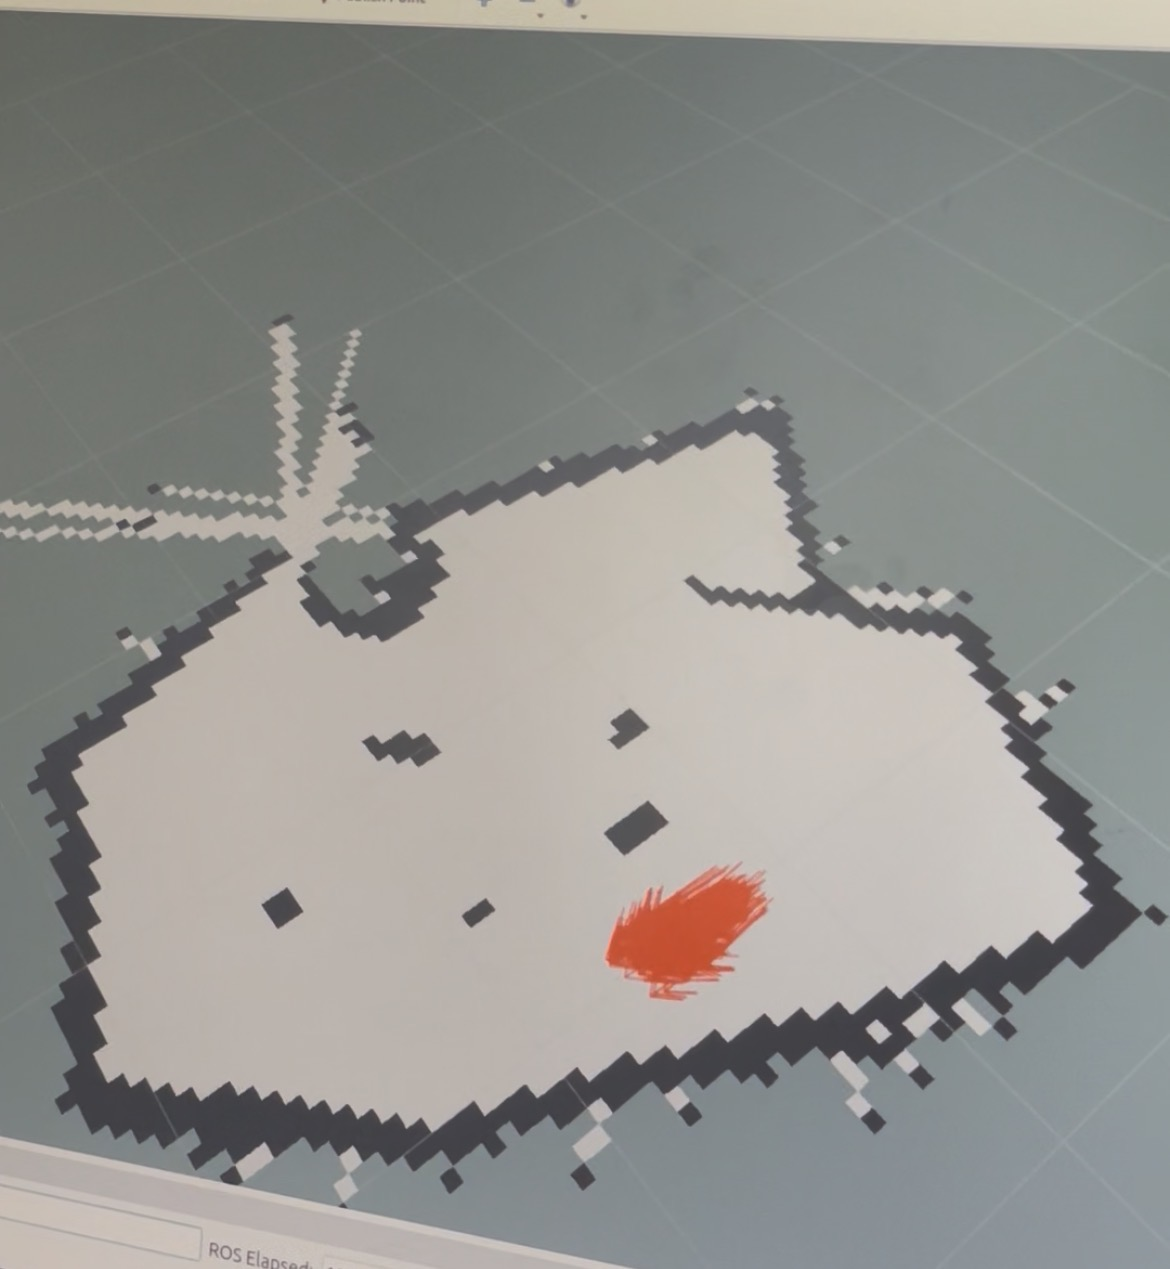
\includegraphics[width=\textwidth]{image.jpg}}{\textit{[AMCL particles screenshot]}}

\vspace{1mm}
{\tiny AMCL particle cloud localizing the robot on the map}
\end{column}
\end{columns}
\end{frame}

% Conclusion
\section{Conclusion}

\begin{frame}{Project Summary}
\begin{block}{What We Accomplished}
$\checkmark$ \textbf{Step 1:} EKF sensor fusion with 110mm average error\\
$\checkmark$ \textbf{Step 2:} Used professional dataset map\\
$\checkmark$ \textbf{Step 3:} AMCL localization successfully implemented
\end{block}

\begin{block}{Key Technical Achievements}
\begin{itemize}
    \item Multi-sensor fusion (odometry + IMU + ground truth at 1Hz)
    \item Real-time error measurement and visualization
    \item Particle filter localization on pre-built map
    \item Complete ROS navigation stack integration
\end{itemize}
\end{block}

\begin{center}
\Large \textbf{Thank you for your attention!} \\
\vspace{0.5cm}
\normalsize Questions?
\end{center}
\end{frame}

\end{document}
